\startchapter{Introduction to the LHC and the ATLAS Detector}
\label{chapter:lhc_atlas}

The Large Hadron Collider (LHC) \cite{lhc_machine} is a circular proton-proton ($pp$) collider which resides in a 27 km tunnel near the European Organization for Nuclear Research (CERN). Superconducting magnets are used to accelerate counter-rotating bunched proton beams to near the speed of light, and direct the beams into head-on collisions at four interaction points around the ring. The collisions take place at a world-leading centre of mass energy of up to 13 TeV. Each interaction point is surrounded by a detector, which measures the energetic debris of particles produced by the high energy collisions to perform precision measurements of the SM and search for new physics.

The large 13 TeV centre of mass energy of the collisions makes it possible for the colliding proton constituents, known as ``partons", to pair annihilate and subsequently produce massive unstable particles such as the Higgs boson, which cannot presently be produced by any other experimental means. Experiments at the LHC can study hypothetical models of physics beyond the SM (``BSM physics") by searching for evidence of the production of the massive particles involved in these models from their subsequent decay to SM particles.

The LHC also collides protons at a world-leading collision rate, $\sim$100 times higher than the next-leading proton collision rate at the Tevatron collider \cite{tevatron} which operated from 1983-2011 and collided protons and anti-protons ($p\bar{p}$) at a peak centre of mass energy of 1.8 TeV. Over several years of data-taking, the high collision rate at the LHC has enabled experiments to collect rich data sets. These large data sets enable searches for new physics to study highly selective subsets of the data in which signatures of new physics are predicted.
%, while still maintaining a sufficient amount of data in these subsets to make statistically significant comparisons with SM predictions to search for excesses in the data that could arise from new physics.

\section{The Parton Model}
\label{sec:parton_model}

Before discussing $pp$ collisions at the LHC in detail, it is important to first introduce the parton model which describes the substructure of protons involved in the collisions. 

The proton has an internal structure comprised of constituent quarks, antiquarks and gluons - collectively known as ``partons" - and their interactions \cite{parton_model}. When a proton collides with another particle in particle colliders such as the LHC, the probability density $f(x, Q^2)$ that a particular species of parton, for example a quark with ``up" flavour $u$, will be involved in the collision is a function of both the fraction $x$ of the proton's momentum carried by the parton, and the squared momentum scale $Q^2$ of the collision. Detailed parameterized models of the parton distribution function (PDF), such as MSHT20 \cite{MSHT20} have been developed using combined fits to data from deep inelastic scattering (DIS) experiments at proton colliders. MSHT20 PDF models at $Q^2$ of 10 GeV$^2$ and $10^4$ GeV$^2$ are shown in Figure \ref{fig:msht20_pdfs}.

\begin{figure}[H]
	\centering
	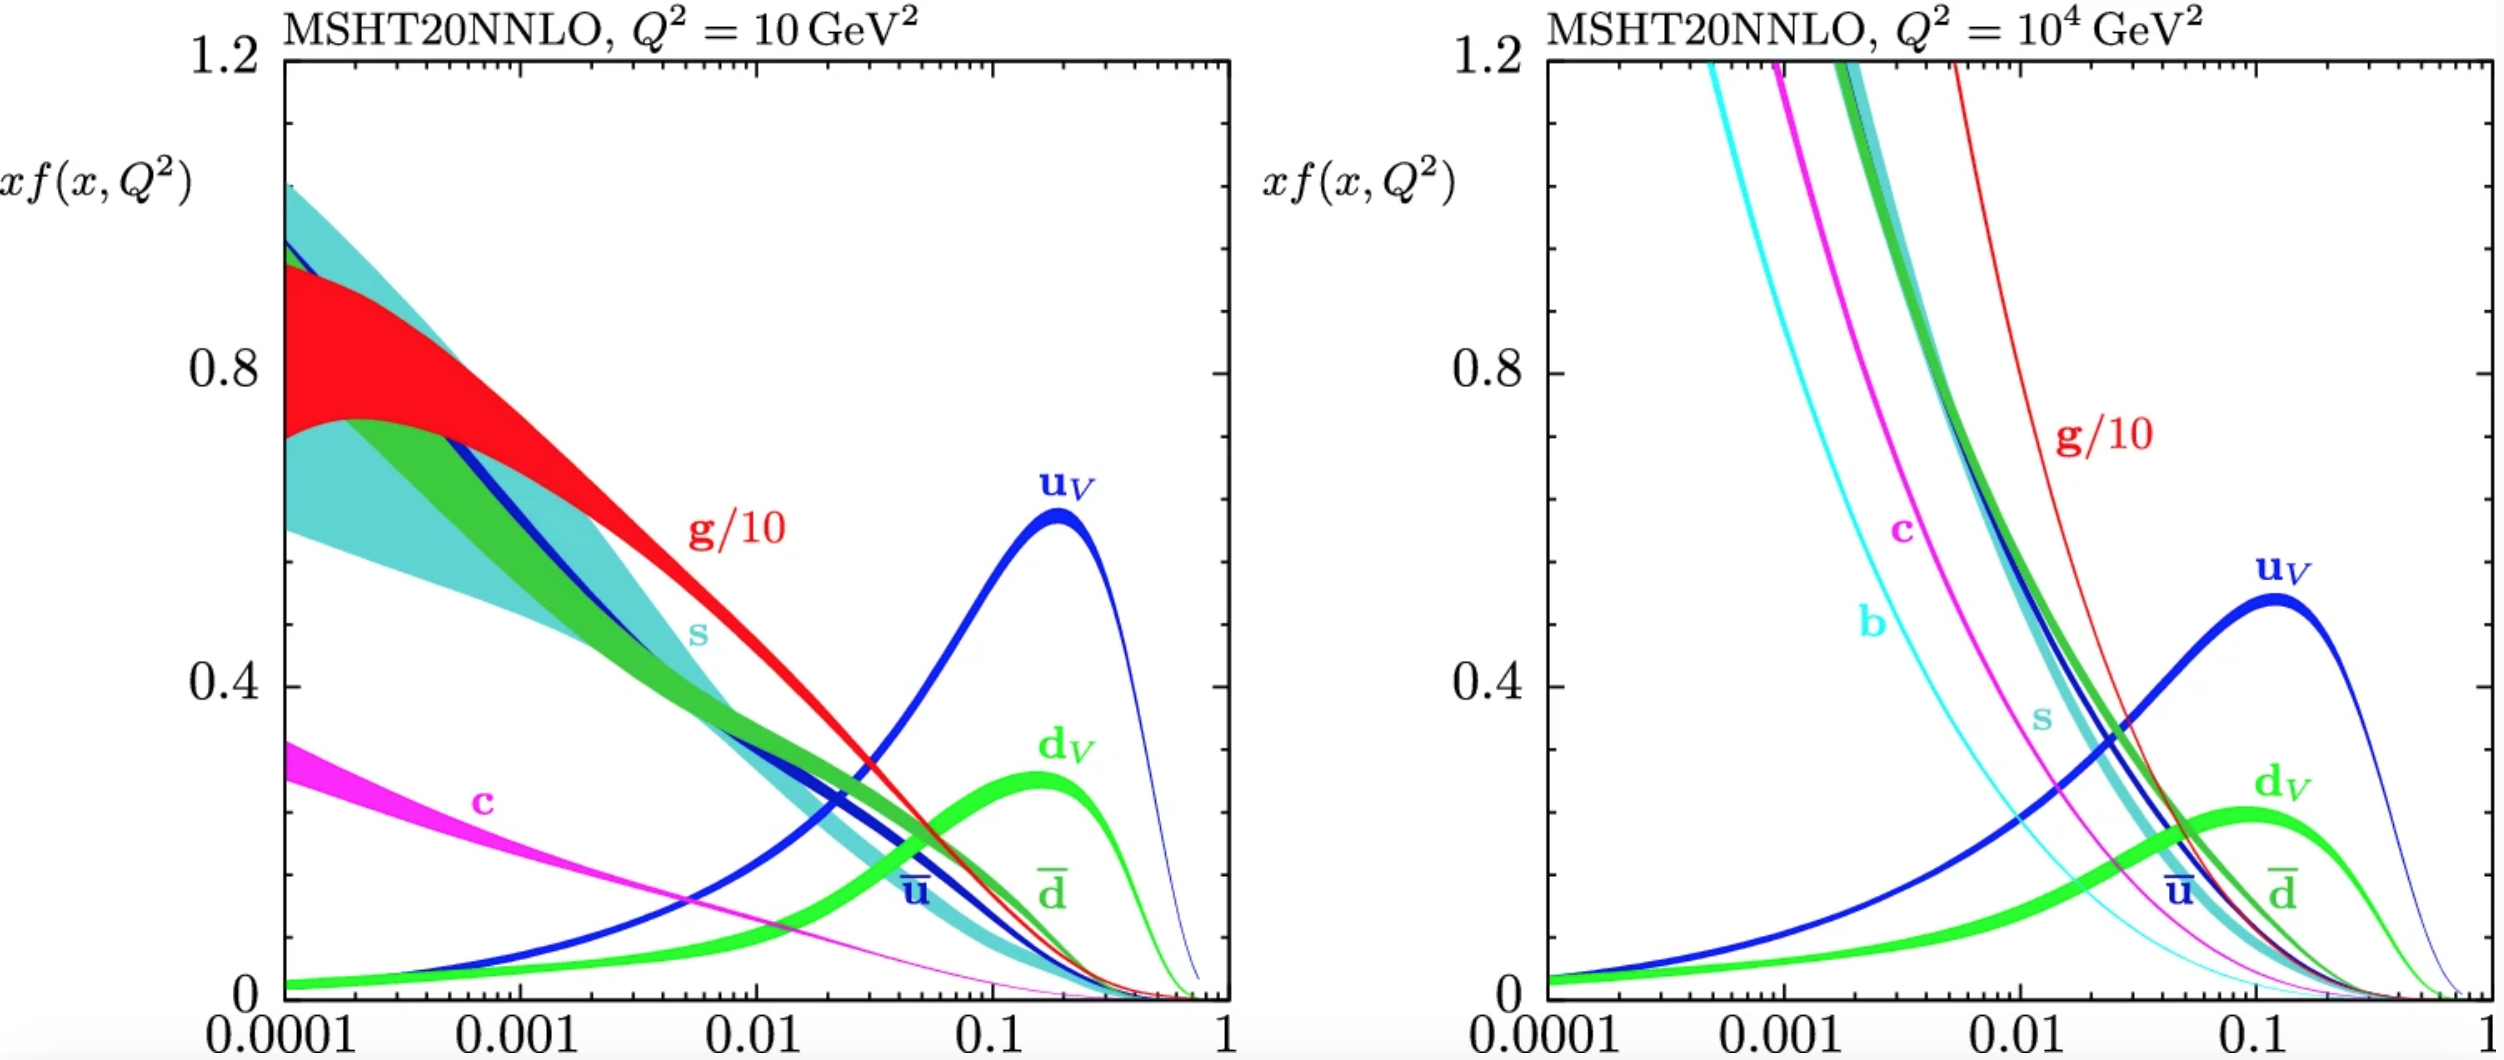
\includegraphics[width=0.9\textwidth]{Figures/3/MSHT20_PDFs.png}
	\caption[]{Parton distribution functions modelled with MSHT20 at $Q^2=10$ GeV$^2$ and $10^4$ GeV$^2$. Figure from $\copyright$ \cite{MSHT20}.}
	\label{fig:msht20_pdfs}
\end{figure}

Based on the PDFs shown in Figure \ref{fig:msht20_pdfs}, $u$ and $d$ quarks carry the highest probability density for parton momentum fractions above $\sim$10\%, with the $u$ carrying approximately double the probability density of the $d$. These dominant quarks are known as the proton's ``valence" quarks, of which there are two $u$ and one $d$, and they carry the proton's quantum numbers.

\section{Decay Processes from Parton Collisions}

Each process of particle production initiated by high-energy particle collisions at the LHC proceeds with a certain probability relative to other processes that could also be initiated by the same collision. The probability that a given process will take place is quantified by its ``cross section" $\sigma$. The beam luminosity $\mathcal{L}$ relates the rate of collisions $\frac{dN}{dt}$ which proceed via a given process to the cross section of the process:

\begin{equation}
\frac{dN}{dt} = \mathcal{L}\sigma
\end{equation}

The luminosity can be integrated over a period of time $t_1$ to $t_2$, such that the total number of events expected to be produced via a process with cross section $\sigma$ over the given period is related to the ``integrated luminosity" $\mathcal{L}_\text{int}$ by:

\begin{equation}
N = \sigma\int_{t_1}^{t_2}\mathcal{L}(t)dt = \sigma\mathcal{L}_\text{int}
\end{equation}

Figure \ref{fig:ATLAS_xsections} shows a summary of cross sections for the production of SM particles - or particle combinations (eg. ``$Wt$" represents the production of a W boson along with a top quark) - from $pp$ collisions at the LHC, as measured by the ATLAS detector \cite{atlas}. 

\begin{figure}[H]
	\centering
	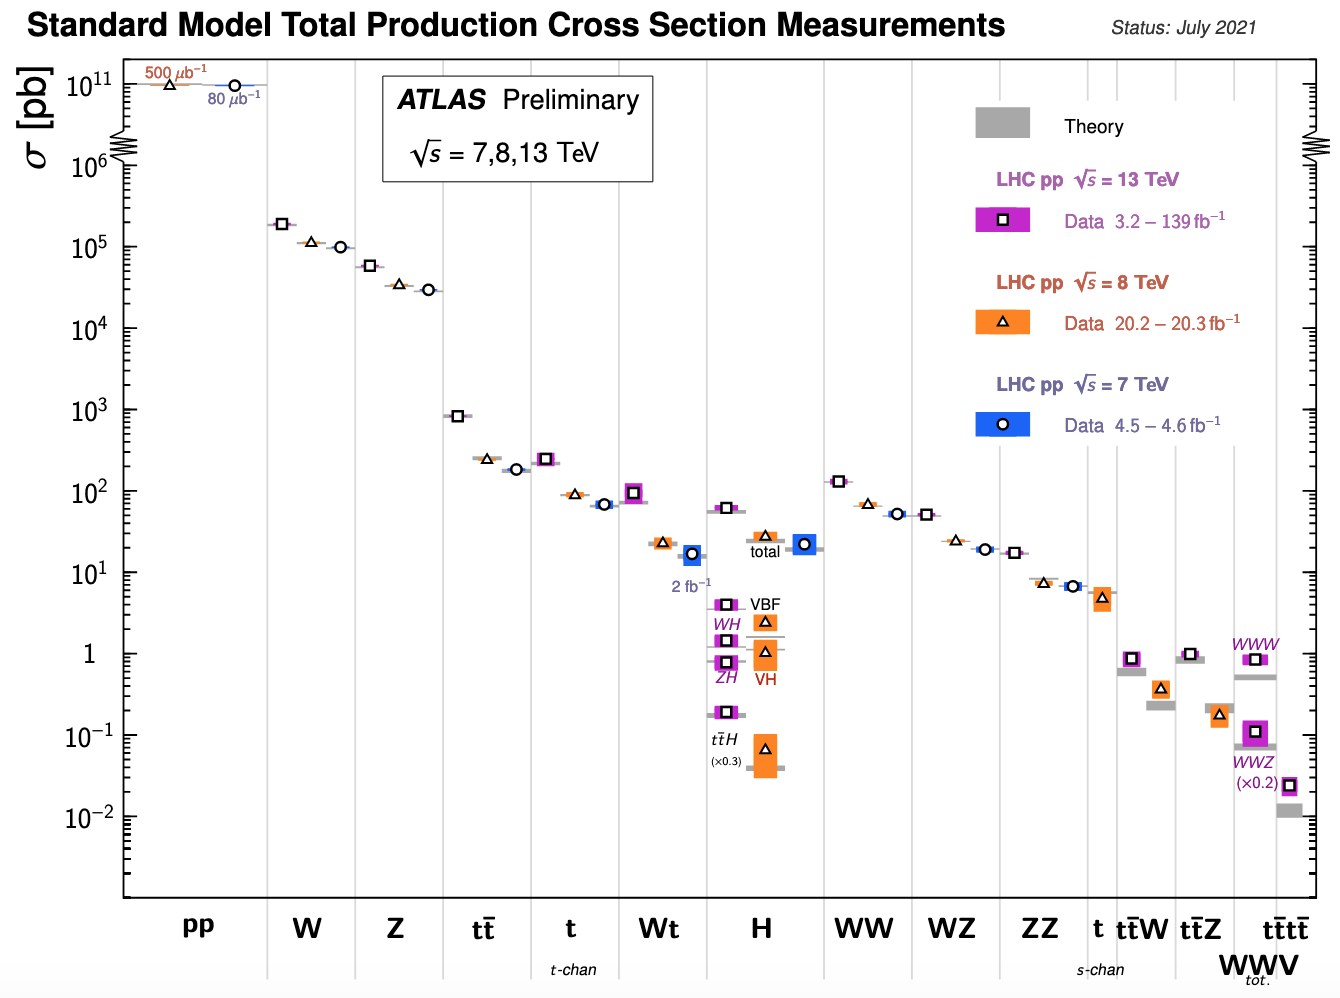
\includegraphics[width=0.9\textwidth]{Figures/3/ATLAS_xsections.png}
	\caption[]{Summary of SM cross sections for particle production processes measured by the ATLAS detector. Figure from $\copyright$ \cite{ATL-PHYS-PUB-2021-032}.}
	\label{fig:ATLAS_xsections}
\end{figure}

\subsection{Branching Fractions and $W$ Boson Decays}

Unstable particles produced by the parton collisions will subsequently decay to less-massive particles, typically with multiple possible mechanisms, also known as ``channels", by which the decay can occur. Each such channel has an associated ``branching fraction", which quantifies the relative probability with which the decay will proceed by the given channel. The search presented in this thesis focuses on DM production in association with a pair of oppositely-charged W bosons. Figure \ref{fig:W_decays} shows the two $W$ boson decay routes. Due to energy and momentum conservation, W bosons can only decay to a pair of particles whose combined mass is smaller than the W mass. Charge conservation additionally requires that the decay products have a combined charge equal to that of the parent W boson. These two requirements allow the W to decay either ``hadronically" to a quark-antiquark pair with one up-type quark/antiquark (U) and one down-type (D), or ``leptonically" to a charged lepton (L) and a neutrino ($\nu$).

%\begin{figure}[H]
%	\centering
%	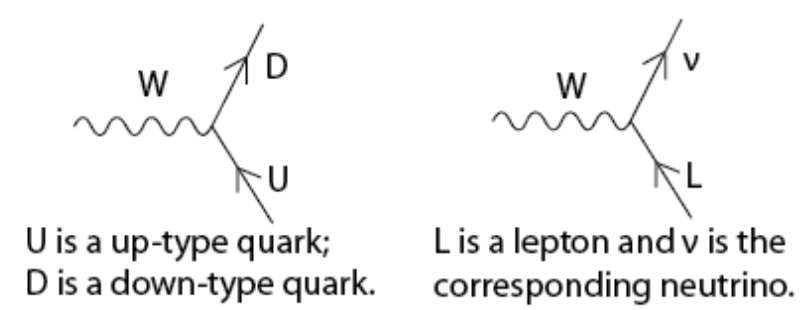
\includegraphics[width=0.5\textwidth]{Figures/3/W_decays.png}
%	\caption[]{W boson decay mechanisms. Adapted from illustration by Garyzx, distributed under a CC BY-SA 3.0 license.}
%	\label{fig:W_decays}
%\end{figure}

\begin{figure}[H]
	\centering
	\begin{subfigure}[b]{0.49\textwidth}
	\centering
		\begin{tikzpicture}
			\begin{feynman}
		 		\vertex (a);
				\vertex at ($(a)+(1.5cm, 0)$) (b);
				\vertex at ($(b) + (0.9cm, 0.75cm)$) (c);
				\vertex at ($(b) + (0.9cm, -0.75cm)$) (d);
		 		
		 		\diagram* {
				(a) -- [boson, edge label'=$W$] (b),
				(b) -- [fermion, edge label=D] (c),
				(d) -- [fermion, edge label=U] (b),
		 		};
		 	\end{feynman}
		 \end{tikzpicture}
	\caption{Hadronic decay mode}
	\label{fig:W_decays_had}
	\end{subfigure}
	\begin{subfigure}[b]{0.49\textwidth}
	\centering
		\begin{tikzpicture}
			\begin{feynman}
		 		\vertex (a);
				\vertex at ($(a)+(1.5cm, 0)$) (b);
				\vertex at ($(b) + (0.9cm, 0.75cm)$) (c);
				\vertex at ($(b) + (0.9cm, -0.75cm)$) (d);
		 		
		 		\diagram* {
				(a) -- [boson, edge label'=\(W\)] (b),
				(b) -- [fermion, edge label=L] (c),
				(d) -- [fermion, edge label=$\nu$] (b),
		 		};
		 	\end{feynman}
		 \end{tikzpicture}
	\caption{Leptonic decay mode}
	\label{fig:W_decays_lep}
	\end{subfigure}
	\caption[]{W boson decay mechanisms}
	\label{fig:W_decays}
\end{figure}

\section{Detectors at the LHC}

The DM search presented in this thesis uses data collected from the ATLAS (A Toroidal LHC ApparatuS) detector \cite{atlas}. ATLAS is one of four particle detectors at the LHC which are designed to measure the energetic debris of particles produced by high energy particle collisions to perform precision measurements of the SM and search for new physics using the resulting particle collision data. This section briefly introduces each of the four particle detectors at the LHC, and what each contributes to the LHC physics programme.

The two largest, \textbf{ATLAS} (A Toroidal LHC ApparatuS) \cite{atlas} and \textbf{CMS} (Compact Muon Solenoid) \cite{cms}, are both general-purpose detectors designed to record all SM decay products from the collisions, with the exception of neutrinos which pass through due to their very low interaction cross sections. Thanks to their near-complete detection of decay products, data from these detectors can be used to study a wide range of physics processes resulting from the collisions, including both measurements of the SM and searches for new physics beyond the SM. By taking a general-purpose approach, rather than specializing in the study of one particular collision or decay process, these experiments seek to maintain sensitivity to the broadest possible range of particle processes, in the hopes of allowing physicists to detect and measure new physics processes in whatever form they may take. While the physics goals of these two detectors are very similar, they are accomplished using different detector designs and technologies, and as such they are able to produce complementary physics results.

The Large Hadron Collider beauty (LHCb) detector \cite{LHCb} is designed to measure heavy quark ($b$ and $c$) decays resulting from $pp$ collisions. Precise measurement of heavy quark decays are of particular interest for the study of CP violation in the SM, and in the search for potential sources of CP violation beyond the SM. Rather than providing full coverage of all collision products, the LHCb detector is comprised of a series of sub-detectors which provide ``forward angle" coverage to detect particles produced with a large boost along the direction of one of the two proton beams. This forward region is of particular interest for measurements of heavy quark decays, because this is the angular region in which heavy quark pairs are predominantly produced by high-energy collisions.

A Large Ion Collider Experiment (ALICE) \cite{ALICE} is designed to measure the products of heavy-ion collisions produced during special LHC runs in which the proton beams are replaced by Pb beams, which are collided at a centre of mass energy of 5 TeV. The high-energy Pb collisions produce a sufficiently high temperature and density to form an unbound state of quarks and gluons known as ``quark-gluon plasma" which would have occurred in the early universe. The study of this exotic state could give novel insights into the theory of quantum chromodynamics which describes interactions that proceed via the strong force, including the phenomena of quark colour confinement and chiral-symmetry restoration \cite{quark_confinement, Karsch:845568}.


\section{Introduction to the ATLAS detector}

The ATLAS detector \cite{atlas}, shown schematically in figure \ref{fig:detector}, is the largest detector by volume to have been built at any particle collider, with a length of 44 m and a height of 25 m, constituting a total weight of approximately 7,000 tonnes. The tremendous amount of detector material is needed to absorb and measure the highly energetic decay products of the $pp$ collisions with sufficient resolution to enable a detailed reconstruction of the particles involved and their kinematic properties. Such a complete and detailed reconstruction of the collisions and subsequent decay processes enable physicists to carry out the impressive range of physics goals shared by the ATLAS and CMS collaborations. These goals include precision measurements of the SM, which profit both from the enormous collision rate, and from the large centre of mass collision energy which enables on-shell production of all known SM particles. The detector is also designed to be sensitive to as wide a range of new physics signatures as possible. Particular emphasis was placed on designing the detector to be sensitive to the anticipated production modes of the Higgs boson, which was jointly discovered by the ATLAS and CMS collaborations in 2012 \cite{atlas_higgs, cms_higgs}. 

The detector provides full 4$\pi$ coverage around the $pp$ interaction point, with the exception of the beam pipe. It consists of several layers of sub-detectors, each of which is specialized for recording specific kinematic information and particle types.

The ATLAS detector is described spatially using the standard coordinate system of $(x,y,z)$ coordinates and ($\theta$, $\phi$) angles shown in Figure \ref{fig:coord_system}. The origin of the coordinate system is placed at the nominal interaction point of the colliding proton beams, and the z axis lies along the beam line. The angle of a particle or detector component in the plane transverse to the beam line is given by the angle $\phi$, and its angle relative to the beam line is given by $\theta$. The ``pseudorapidity" $\eta$ is a quantity related $\theta$ according to:

\begin{equation}
\label{eq:pseudorapidity}
\eta=-\ln\Big[\tan\Big(\frac{\theta}{2}\Big)\Big]
\end{equation}

Pseudorapidity is often used rather than $\theta$ because differences $\Delta\eta$ in pseudorapidity are invariant under Lorentz boosts along the z axis.

\begin{figure}[H]
	\centering
	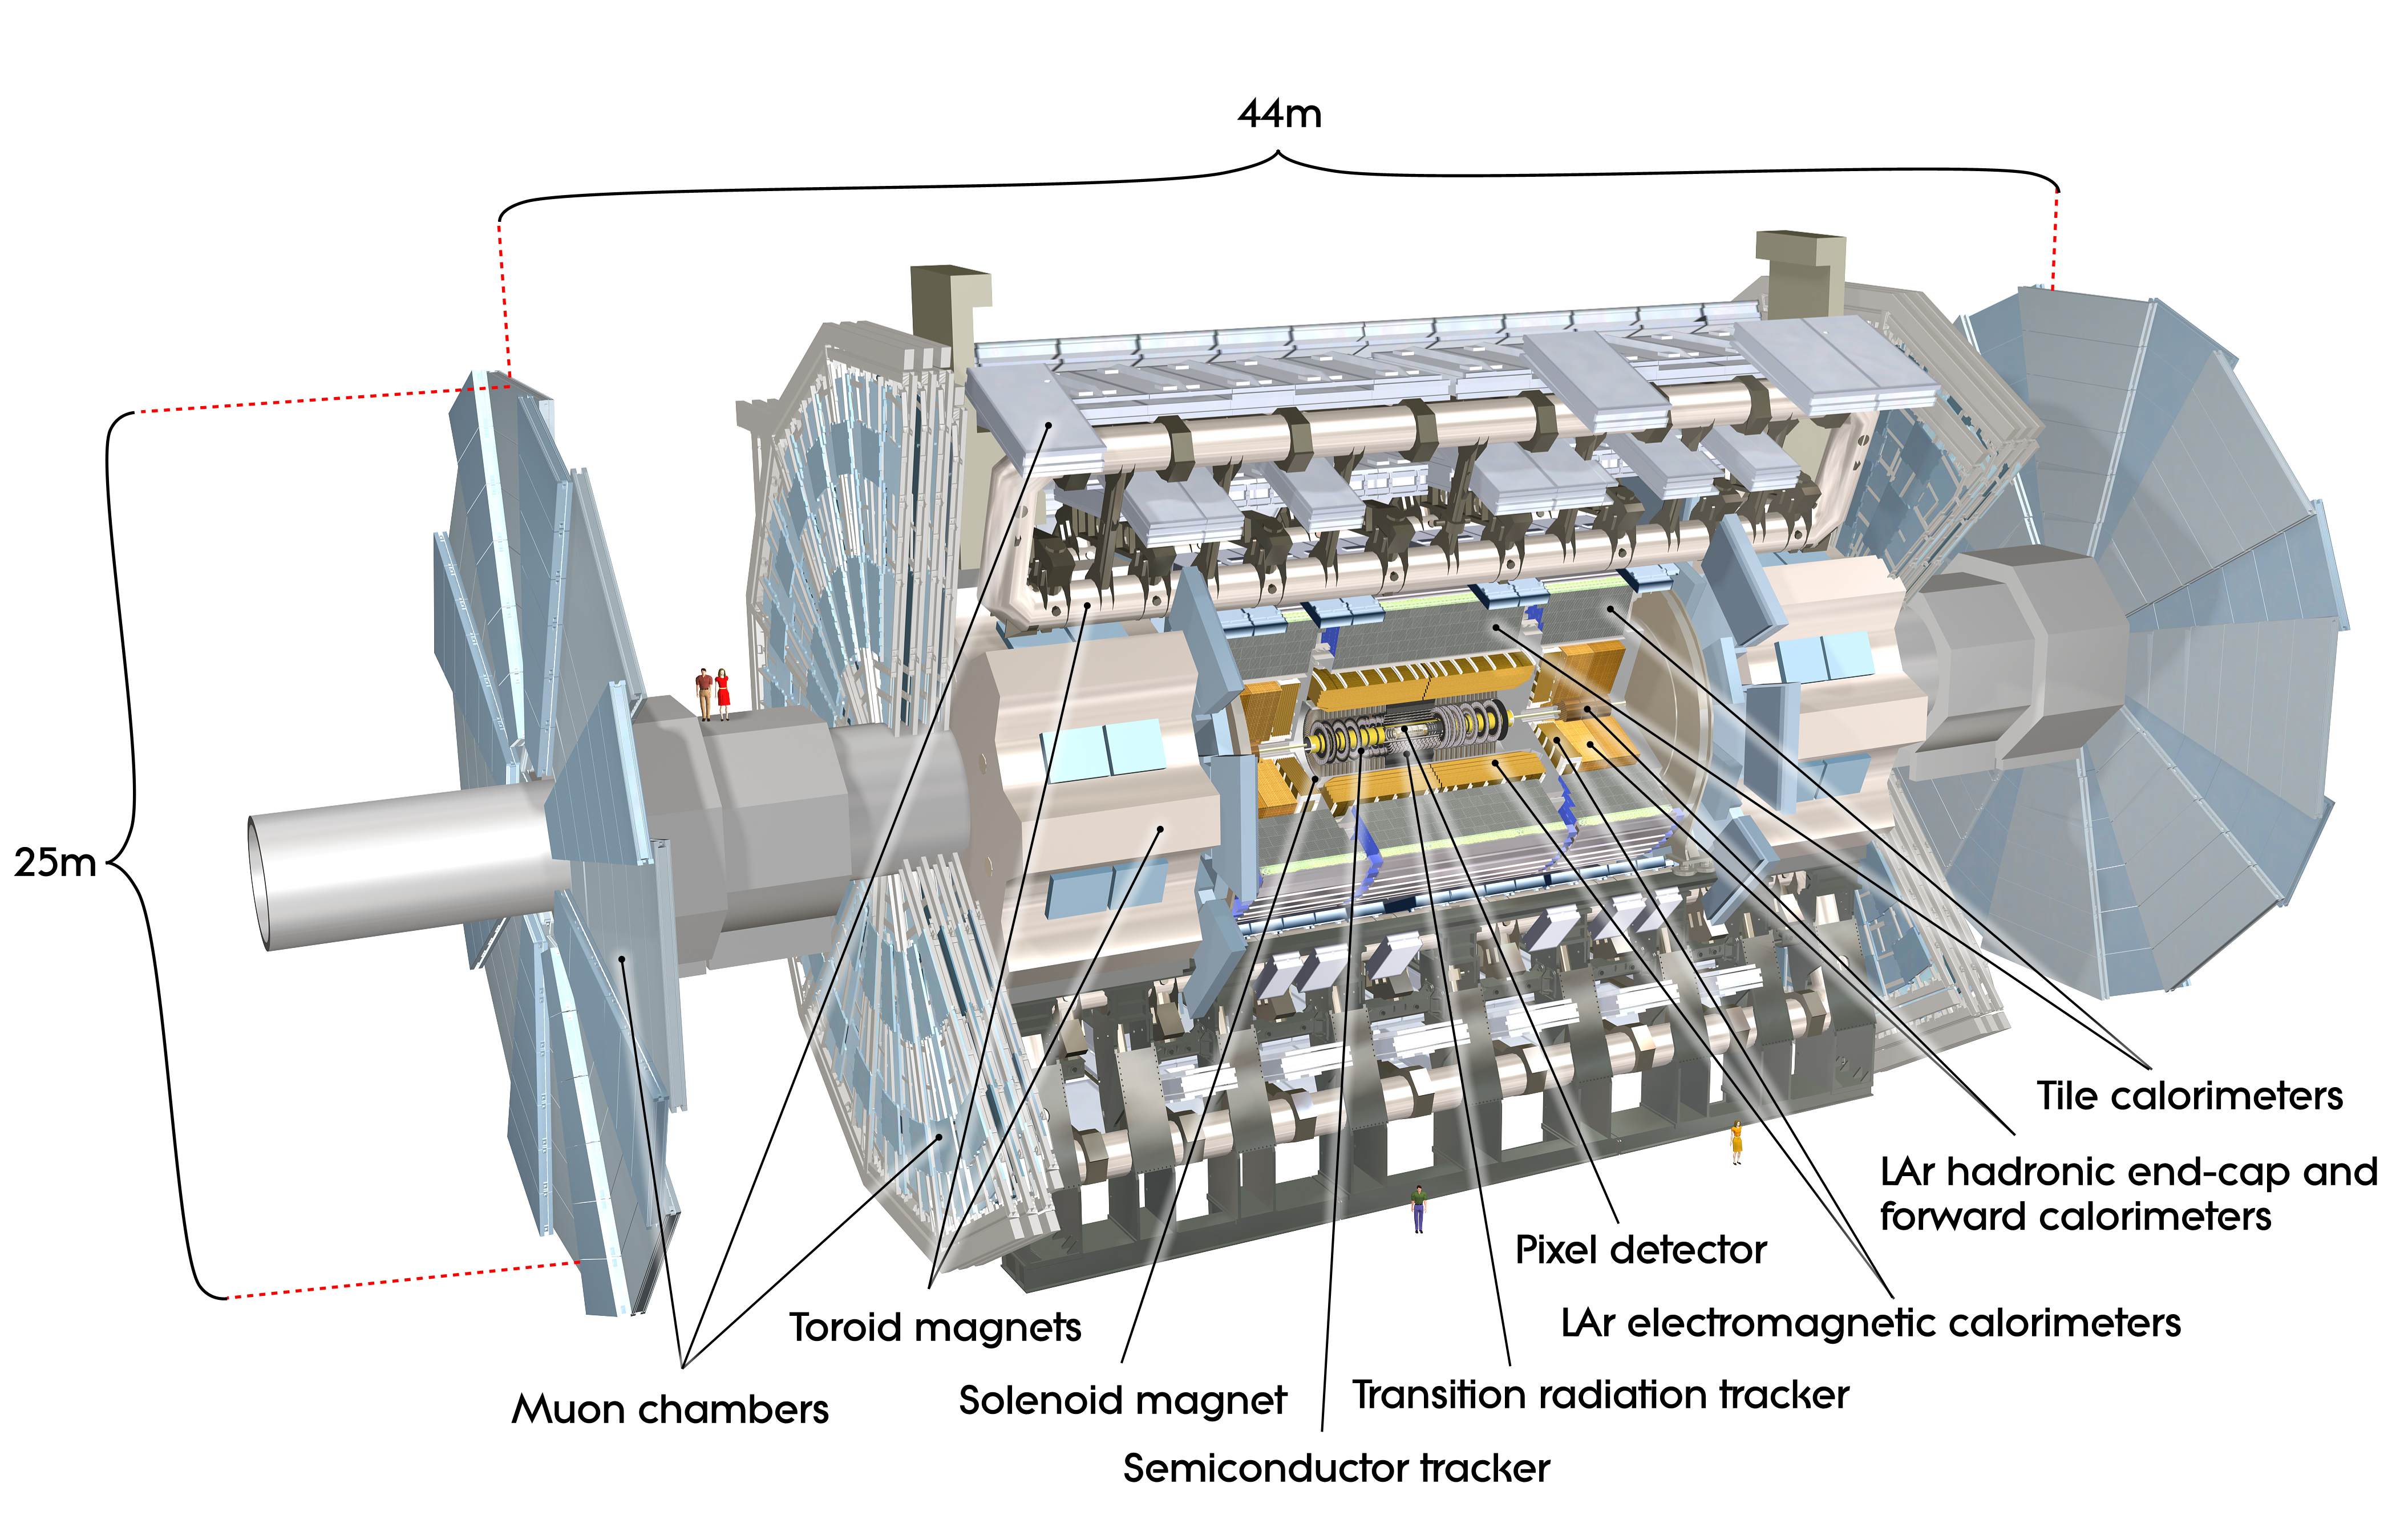
\includegraphics[width=0.85\textwidth]{Figures/3/detector.jpg}
	\caption[]{Schematic diagram of the ATLAS detector. Figure from $\copyright$ \cite{atlas}}
	\label{fig:detector}
\end{figure}

\begin{figure}[H]
	\centering
	\begin{subfigure}[b]{0.45\textwidth}
	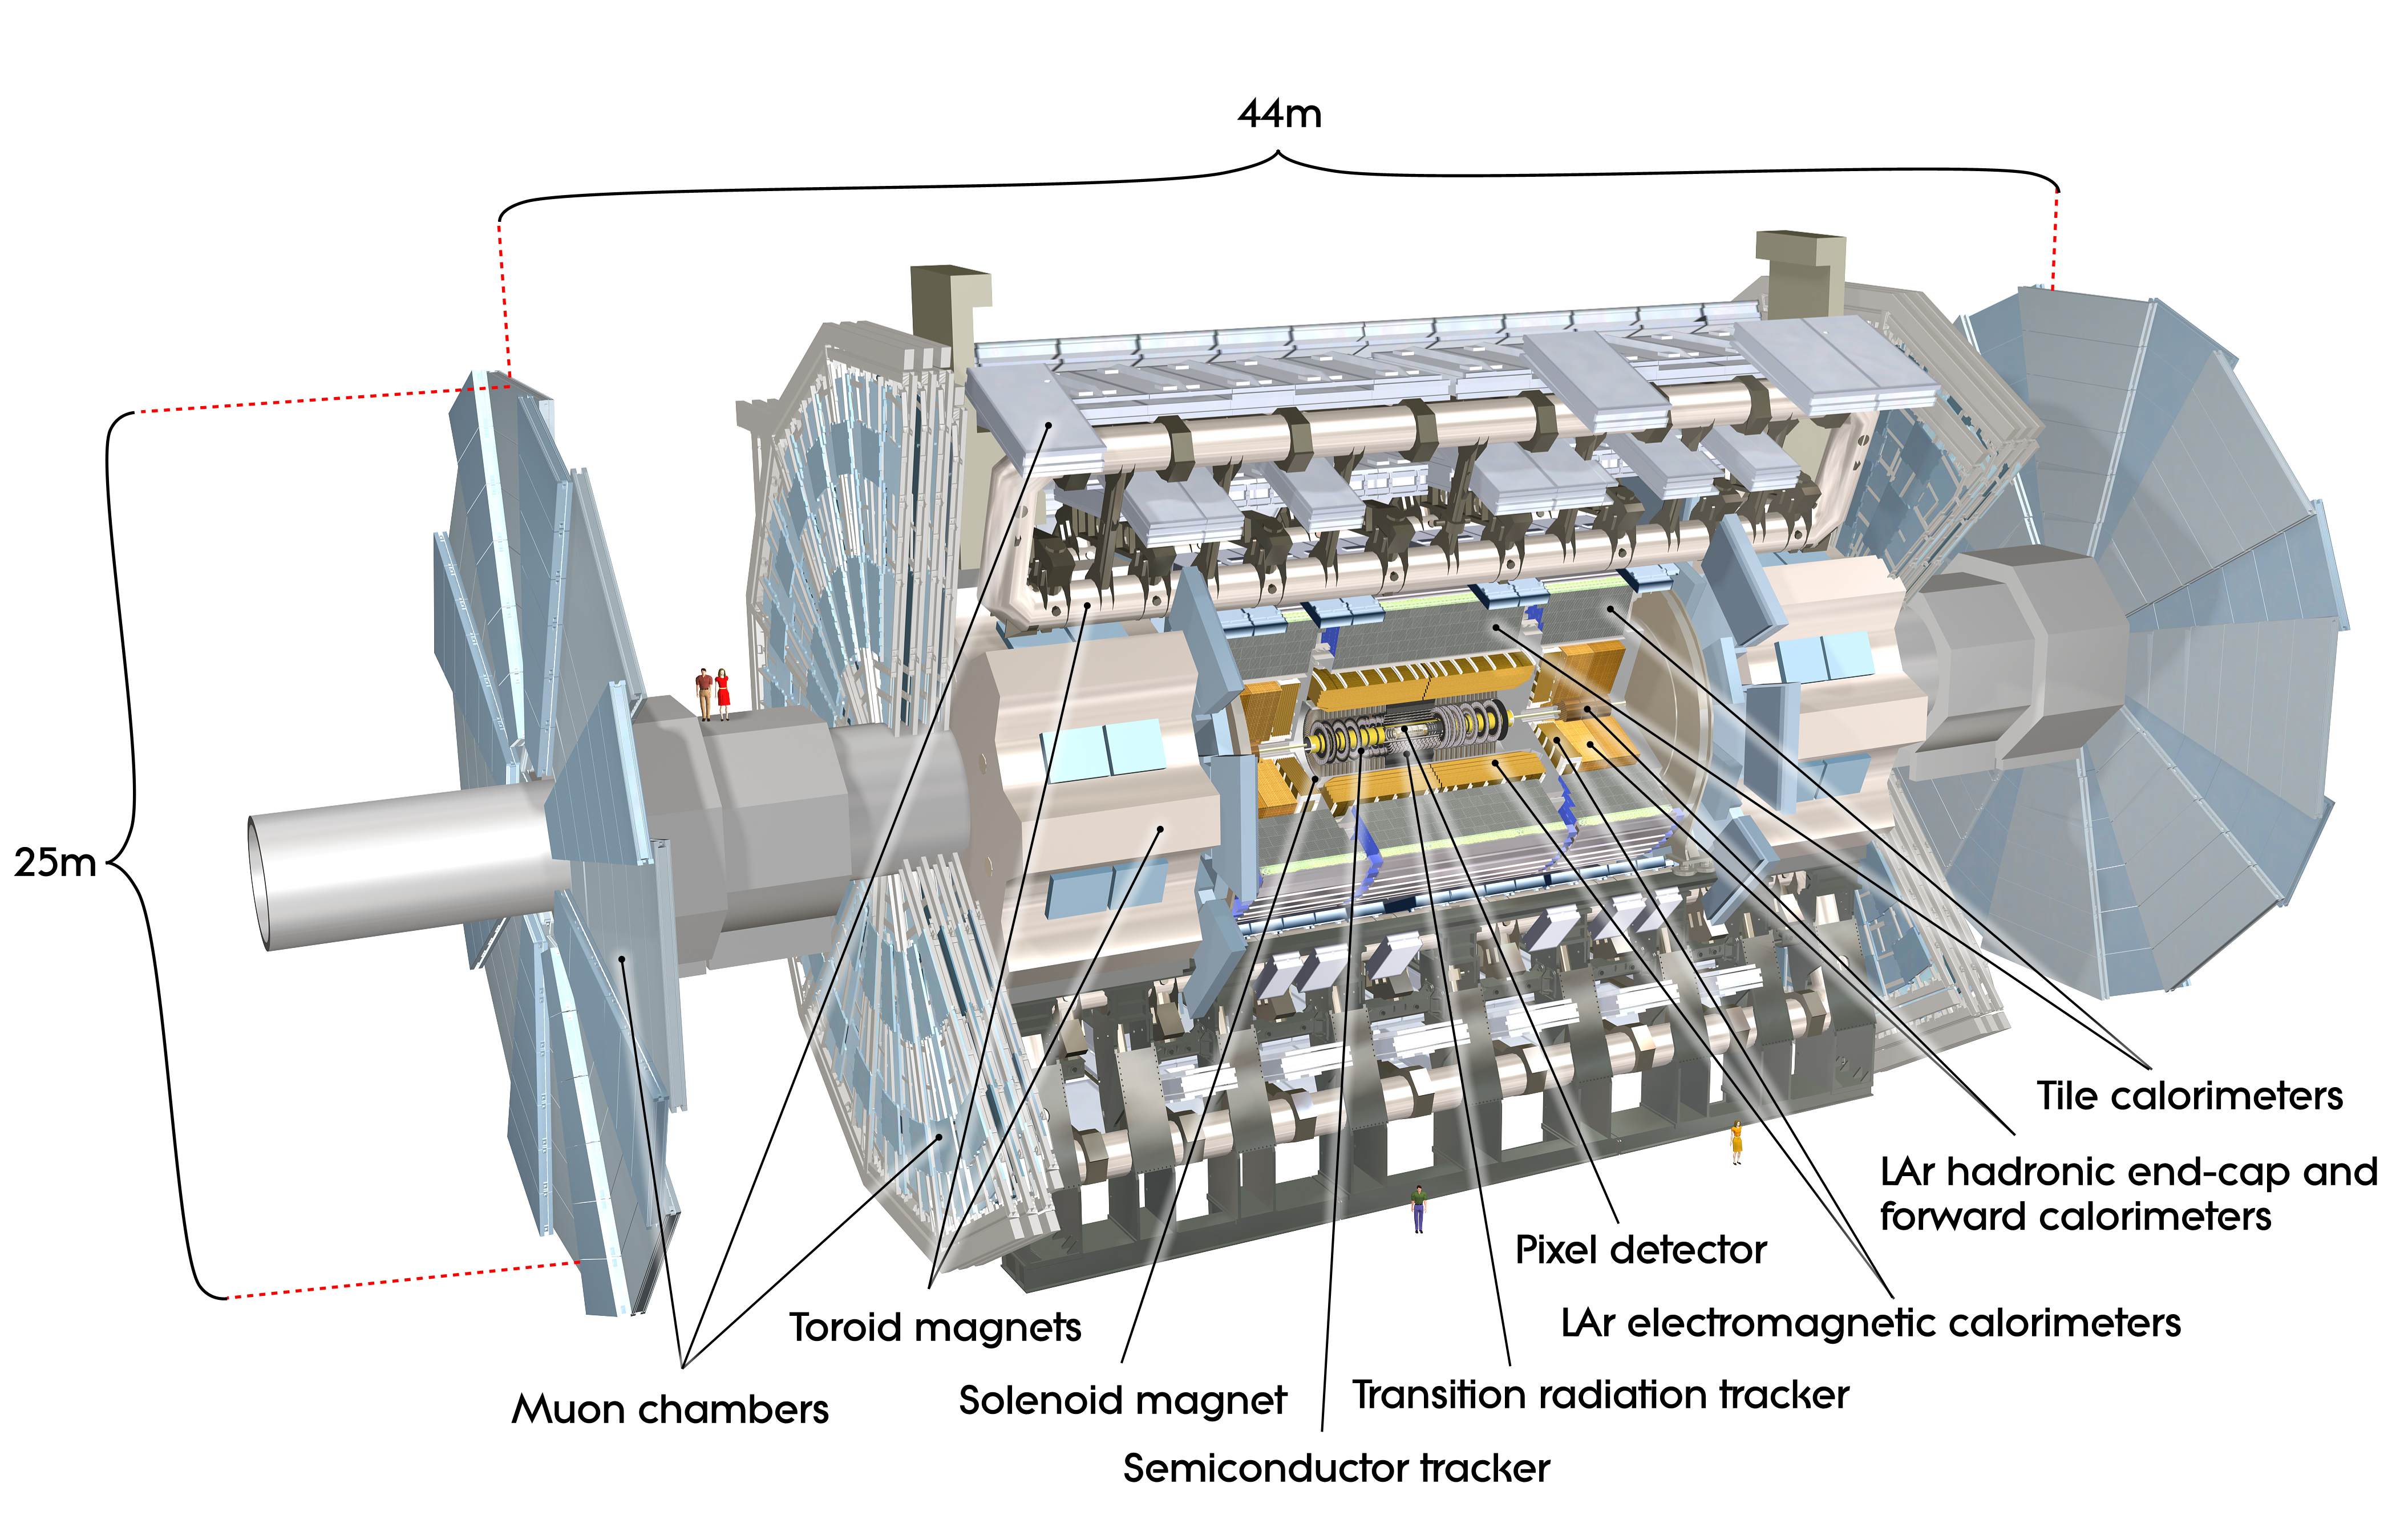
\includegraphics[width=0.9\textwidth]{Figures/3/detector.jpg}
	\caption{ATLAS Detector}
	\label{fig:detector}
	\end{subfigure}
	\begin{subfigure}[b]{0.45\textwidth}
	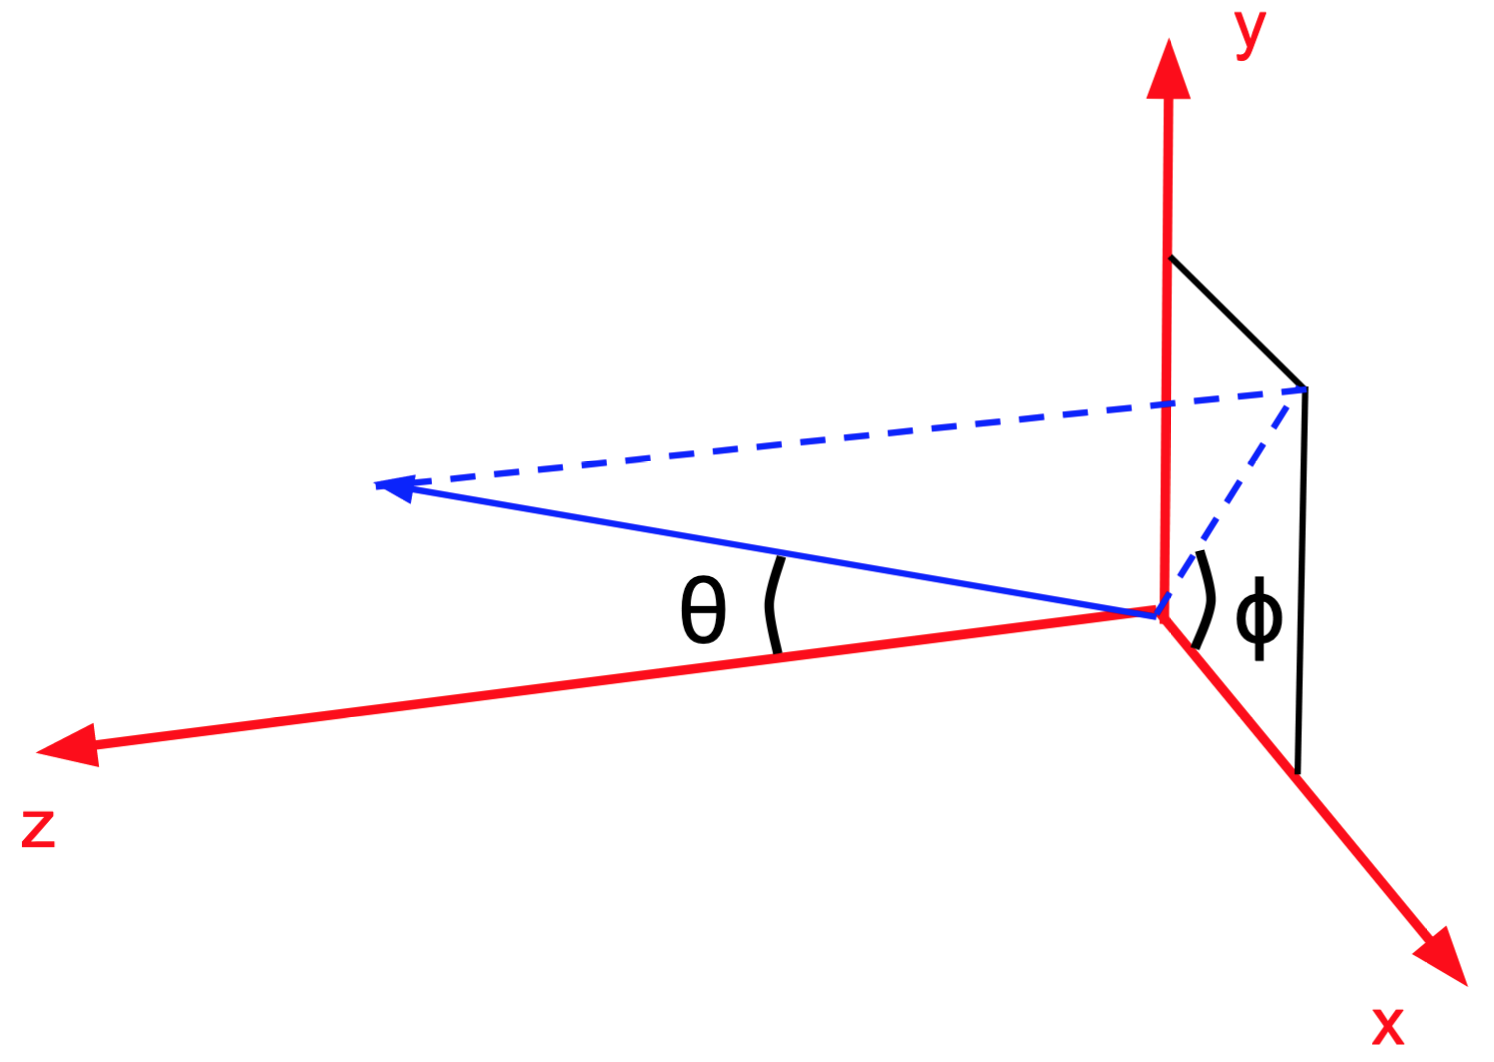
\includegraphics[width=0.8\textwidth]{Figures/3/ATLAS_coordinate_system.png}
	\caption{Standard coordinate system for the ATLAS Detector}
	\label{fig:coord_system}
	\end{subfigure}
	\caption[]{Left: Schematic diagram of the ATLAS detector (figure from $\copyright$ \cite{atlas}). Right: Standard coordinate system used for the ATLAS detector.}.
	\label{fig:detector}
\end{figure}

The ATLAS sub-detectors are described in some detail in the following sections.

\subsection{The Inner Detector}

The inner detector (ID), located nearest the beam pipe, is specialized for charged particle tracking. It is immersed in a 2T magnetic field oriented parallel to the beam pipe, which bends the trajectories (``tracks") of electrically charged particles as they pass through the field. Three distinct but complementary high-resolution tracking technologies are employed along with pattern recognition tools to map the trajectories of charged particles passing through the ID. The tracking is accomplished with as little material as possible in the ID, such that the particle trajectories can be mapped with minimal scattering and energy loss before they reach the calorimeters \cite{id_thesis}. 

Tracks from the inner detector are reconstructed by assembling clusters of ``hits" in channels of the ID tracking layers \cite{electron_reco}. The reconstructed tracks are a critical component of vertex reconstruction, and the degree of bending and direction of the bent tracks at the production vertex provide information about the momentum, charge, and identity of the charged particles that produced them. 


\subsection{The Calorimeters}

The calorimeter is designed to measure the energy of all particles which pass through it by initiating cascades of secondary particle production in the high-density detector material known as ``showers", and fully absorbing the energy of each shower. The only particles which cannot be absorbed by the calorimeter are muons and neutrinos, which pass through without showering. The calorimeter is divided into two sub-detectors, the electromagnetic and hadronic calorimeters. Both are ``sampling calorimeters", which means they are comprised of repeated layers of dense absorbing material with ``sampling" layers in between. The sampling layers track the location of the shower and record a small fraction of its energy, to which a calibration factor is applied to infer the full shower energy. 

\subsubsection{The Electromagnetic Calorimeter}
\label{sec:EM_calo}

The electromagnetic (EM) calorimeter forms the inner calorimeter layer, and is designed to fully absorb and measure the energies of electrons, positrons and photons. Energy is primarily deposited in the lead absorbing layers in the form of EM showers \cite{em_showers}, in which the initial electron or photon interacts via bremsstrahlung \cite{shower_theory} with the absorbing material to produce a cascade of photon radiation and electron pair production. The sampling layers are filled with liquid argon (LAr), which absorbs relatively little energy compared with the lead absorbing layers due to its lower density. Ionization is produced when a charged particle passes through the LAr \cite{em_cal} layer, which drifts through an electric field generated by a high voltage placed between absorber plates and readout electrodes on either end of the LAr layer to produce a triangular current pulse \cite{LAr_calo}. 

Candidate EM showers (``clusters") are reconstructed from energy deposits in calorimeter cells using a ``seed-cluster" algorithm described in Ref. \cite{electron_reco}. The seed-cluster algorithm works by dividing the $\eta\times\phi$ space of the EM calorimeter into a grid of $\eta\times\phi=0.025\times0.025$ solid angle elements called ``towers". For each such element, the energy detected in all the calorimeter layers which lie within the given patch of solid angle is summed to form the energy of the tower. A sliding window algorithm of size $3\times5$ towers is used to construct energy clusters which constitute EM clusters from localized energy deposits.

Reconstruction and selection of electron candidates \cite{electron_reco} is performed with the use of a complex matching algorithm to match candidate reconstructed tracks in the ID with EM clusters in the calorimeter based on their proximity in $\eta\times\phi$ space. This matching is complicated by the fact that electrons may radiate photons via bremsstrahlung in the ID prior to reaching the calorimeters. The radiated photons can subsequently decay into an electron-positron pair, which themselves can generate tracks in the ID. As a result, it is possible to reconstruct multiple tracks in the ID, all originating from the same electron, and match these tracks to EM clusters in the calorimeter. In case several tracks in the ID can be matched to the same EM cluster, the track considered to be associated with the primary electron is selected by an algorithm that accounts for, among other quantities, the number of hits in the ID and the distance in $(\eta, \phi)$ between the extrapolated track position in the calorimeter and the barycentre of the EM cluster. 

Reconstructed objects selected as electron candidates are subsequently passed through a likelihood-based electron identification algorithm, described in detail in Section 6 of Ref. \cite{electron_reco}, which uses as a discriminant the ratio 

\begin{equation}
\label{eq:electron_likelihood_id_discriminant}
d_L = \frac{L_S}{L_S+L_B}
\end{equation}

\noindent where the likelihood function $L_S(B)$ is a product of signal (background) PDFs for various quantities related to the reconstructed object such as track conditions, details of the track-cluster matching, and reconstructed EM shower widths for the EM cluster in various layers of the EM calorimeter. The signal $S$ is ``prompt" electrons, which originate from the primary interaction, and the background $B$ is a combination of jets that mimic prompt electron signatures, electrons from photon conversions in the detector and non-prompt electrons originating from hadron decays.

\subsubsection{The Hadronic Calorimeter}

The vast majority of collision events that occur in the ATLAS detector ultimately result in the production of quarks and gluons. Due to the phenomenon of colour confinement, quarks and gluons cannot exist in isolation, and immediately ``hadronize" to form colour-neutral combinations of quarks called ``hadrons". As these hadrons pass through the detector, they eventually undergo a showering process similar in principle to the EM showers described in Section \ref{sec:EM_calo}. In the case of these ``hadronic showers", the shower is initiated by the strong interaction of a hadron with the detector material to produce a cascade of secondary hadrons \cite{shower_theory}. Unlike the EM showers which proceed exclusively via electromagnetic interactions, hadronic showers proceed via both the strong and EM interactions, where the EM interactions are primarily induced by electromagnetic decays of neutral pions ($\pi^0$) \cite{shower_theory}. Because hadronic showers involve strong interactions, they are in general much more complex in terms of the variety of particles and mechanisms involved in the showering, and as a result are in general more variable and less localized compared with EM showers.

The hadronic calorimeter surrounds the EM calorimeter, and is designed to fully absorb and measure hadronic showers. The primary hadrons which initiate these hadronic showers generally pass through the EM calorimeter without showering due to their relatively long interaction length \cite{atlas}. The hadronic calorimeter is comprised of a tile calorimeter which encircles the EM calorimeter barrel, and a LAr calorimeter with copper and tungsten absorbers in the end-cap region which encloses the two ends of the barrel. The tile calorimeter uses steel as the absorber material and scintillators read out by photomultiplier tubes (PMTs) in the sampling layers. 

Hadronic showers are reconstructed as ``jets" using clusters of energy deposited in the hadronic calorimeter cells \cite{jet_reco}. The jets can be reconstructed using a variety of different reconstruction algorithms depending on the use case. 

Most jet reconstruction algorithms use clusters of topologically connected calorimeter cells known as ``topo-clusters" as basic building blocks for jet reconstruction. Topo-clusters are designed with the goal of extracting significant signals of energy deposition originating from energetic hadrons from the background of detector noise and other sources of fluctuation in the calorimeter cells. Candidate clusters are formed from ``seed cells" in which the deposited energy $E$ is $E>S\sigma_\text{cell}$, where $\sigma_\text{cell}$ is the average noise for the given cell and $S$ is the ``seed threshold" significance, set to 4 by default \cite{topo_cell_clustering}. Cluster construction proceeds by collecting neighbouring cells with energy $E>N\sigma_\text{cell}$, where $N$ is the ``growth threshold", set to 2 by default. If a neighbouring cell passes the $E>N\sigma_\text{cell}$ requirement, its neighbours will also be added to the cluster if their energy significance exceeds the growth threshold, and this process repeats until there are no remaining neighbouring cells with significance above the growth threshold. Lastly, one set of neighbouring cells which satisfy $E>P\sigma_\text{cell}$ are added to the cluster, where $P$ is the ``principal cell filter", set to 0 by default.

Jets are reconstructed from these topo-clusters using the anti-$k_t$ clustering algorithm described in Ref. \cite{akt_algo} in a cone with an angular radius $R$ in $(\eta, \phi)$ space, given by:

\begin{equation}
\label{eq:jet_radius}
R = \sqrt{\eta^2 + \phi^2}
\end{equation}

The jet radius $R$ determines the angular radius within which the anti-$k_t$ algorithm will include calorimeter deposits in the vicinity of a topo-cluster or a set of topo-clusters and attempt to group the energy deposits into jets. Different choices of $R$ can be used in the algorithm depending on the identity and kinematics of the shower parent particle(s) that one is interested in reconstructing \cite{jet_reco}. Jets produced by quarks and gluons which either originate from different parent particles, or whose shared parent particle has a relatively low momentum in the lab frame (a.k.a. ``low boost"), generally have sufficient angular separation that they can be individually reconstructed using relatively small radius parameters such as $R=0.2$ or $R=0.4$. 

Jets which originate from boosted massive particles, such as the hadronically decaying $W$ boson in the search presented in this paper, generally contain two or more significant topo-clusters (a.k.a. ``prongs") in close angular proximity, each having been induced by the hadronization of a strongly interacting daughter particle produced by the hadronic decay of the massive parent particle. In this latter case, the angular proximity of these significant topo-clusters can make it challenging to usefully reconstruct them as individual small-radius jets due to the resulting jet overlap. In these cases, it may be more useful to capture all the decay products in a single jet reconstructed with a larger radius parameter such as $R=0.8$ or $R=1.0$, such that the resulting large-radius jet fully reconstructs the massive parent particle. Methods such as the TAR algorithm \cite{TAR_algo} employed in this analysis are subsequently applied to the reconstructed large-radius jet to obtain useful jet sub-structure information, including the likely number of prongs contained within the jet.

\subsection{The Muon Spectrometer}

The muon spectrometer \cite{atlas} surrounding the calorimeter is specialized for tracking muons and measuring their momentum. It employs the same principle used in the inner detector of applying a strong magnetic field and measuring the resulting bent trajectories of the electrically charged muons passing through to infer their momenta. 

The magnetic field is generated by rectangular superconducting ``toroid magnets" arranged azimuthally in radial planes around the beam axis, which set up a toroidal field concentric to the beam axis. In the region containing the strong field established by the toroid magnets, muon tracks are recorded by three cylindrical layers of muon tracking chambers in the barrel region and three layers of chambers arranged in wheels perpendicular to the beam axis in the end-cap region. Additional layers of fast trigger chambers deliver muon track information to the ATLAS trigger system (see Section \ref{sec:trigger}) so it can be incorporated into the event readout decision. 

Precise measurements of muon track coordinates are provided by monitored drift tubes (MDTs) in the barrel region, which cover a pseudorapidity range of $|\eta|<2.0$), and by cathode strip chambers (CSCs) in the end-cap region ($2.0<|\eta|<2.7$). The CSCs are designed to withstand the relatively high flux of energetic particles which bombard the detector in the end-cap region. These MDTs and CSCs measure track coordinates with nominal resolutions of 60 $\mu$m and 80$\mu$m, respectively, in the magnetic bending plane \cite{muon_reco}. 

High precision tracking is needed both to achieve the design performance goal of reconstructing muon transverse momenta with at most 10\% resolution for 1 TeV tracks \cite{atlas}, and to distinguish prompt muons which originate from the primary interaction from the background of non-prompt muons which arise from secondary interactions in the detector. Reconstruction and identification of prompt muons is performed by combining tracking information from the muon spectrometer and the inner detector, along with energy deposition measurements from the calorimeters. Various muon reconstruction strategies are employed, which attempt to match tracks between the muon spectrometer and the inner detector, or to match inner detector tracks with calorimeter deposits \cite{muon_reco}.

\subsection{Missing Transverse Momentum}
\label{sec:met}

Many signatures of hypothesized processes involving physics beyond the SM - including the DH model considered in this thesis - involve the production of particles which would pass through the ATLAS detector without being detected due to their extremely low interaction cross section with SM particles. Similarly, neutrinos produced in weak interactions will also pass undetected for the same reason. 

The law of momentum conservation, which requires the vector sum of momenta of all measured particles produced by a collision to match that of the initial state quarks, can be used to infer the presence of undetected particles in the collision. Because the fraction of proton momentum carried by each of the initial state quarks - described by the PDFs presented in Section \ref{sec:parton_model} - is statistical in nature, the momenta in the direction of the $pp$ beam line cannot be known precisely. However, initial state quark momenta in the plane transverse to the beam line are in general negligibly small compared with the collision energy, so it can be expected to a high degree of precision that the final state particle momenta in this transverse plane will sum to zero. This expectation implies that collision events which produce undetected particles with an appreciable momentum in the transverse plane can be expected to exhibit a signature of high missing transverse momentum in the final state. 

This two dimensional missing transverse momentum vector for a collision event is typically denoted ``\metvec", and its magnitude ``\met". The components  of \metvec lie in the transverse $(x, y)$ plane of the detector, and are given by:

\begin{equation}
\label{eq:met_components}
E_{x(y)}^\text{miss} = -\sum_i p_{x(y), i}
\end{equation}

\noindent where the sum is over all fully reconstructed electrons, muons, photons, hadronically-decaying tau leptons and jets (a.k.a. ``hard objects"), and additionally over all other detector signals which were recorded as part of the event, but were not used as part of the construction of the hard objects (a.k.a the ``soft term") \cite{met_reconstruction}.

\noindent \metvec and \met are constructed from the components $E^\text{miss}_{x(y)}$ as follows:

\begin{equation}
\label{eq:met_vec}
\metvec = (E^\text{miss}_{x}, E^\text{miss}_{y})
\end{equation}

\begin{equation}
\label{eq:met_mag}
\met = |\metvec| = \sqrt{(E^\text{miss}_{x})^2 + (E^\text{miss}_{y})^2}
\end{equation}

\subsection{The Trigger System}
\label{sec:trigger}

An overwhelming majority of collision events in the ATLAS detector result in ``soft quantum chromodynamics" (soft QCD) interactions which proceed via the strong force and produce only quarks and gluons which have a relatively low momentum in the lab frame - and hence are referred to as ``soft" - and which do not result in the production of any high-mass ($\mathcal{O}(\text{GeV})$) particles. Figure \ref{fig:detector} compares the overall cross section of all interactions resulting from $pp$ collisions with the cross sections of processes which produce various massive SM particles. The overall collision cross section is $\sim$6 orders of magnitude larger than the highest cross section for producing a massive particle, namely that of the $W$ boson. The soft QCD interactions which dominate the total cross sections are in general not of interest for the ATLAS physics programme. It would be impossible to process and save all collision events produced in the ATLAS detector, as the massive flux of these soft QCD interaction events would very quickly overwhelm the bandwidth of the data acquisition system and fill up the available offline data storage capacity. 

The ATLAS trigger \cite{ATLAS_Trigger} is designed to efficiently select a tiny minority of collision events to be read out, processed and saved to offline storage (a.k.a. ``recorded") based on a set of criteria applied to preliminary event information from the sub-detector. The criteria are designed to select for signatures from the sub-detectors that are considered likely to represent processes that will be of interest to the various analyses which study the data either to measure parameters of the SM, or to search for evidence of BSM physics.

The trigger system is divided into a hardware-based ``first level trigger" (L1 trigger) and software-based ``high-level trigger" (HLT), which collectively select events at an average rate of $\sim$1000 Hz from the total collision rate of 40 MHz \cite{ATLAS_Trigger}. Events must be accepted by both the L1 trigger and the HLT in order to be recorded.

The L1 trigger is based on candidate objects identified within regions of interest (``RoIs") defined by their $\eta$ and $\phi$ ranges. Candidate objects are divided into muons, EM calorimeter clusters, jets in the hadronic calorimeter and taus. In addition, the sums of missing transverse momentum (\met) and total energy are also constructed. Hardware level trigger decisions are designed using combinations of these reconstructed objects and sums. Events which pass the L1 trigger are subsequently processed by the HLT. The L1 trigger is designed to form the ``trigger decision" of whether to reject the event or accept it for processing by the HLT within at most 2.5 $\mu$s per event \cite{ATLAS_Trigger}. 

Thanks to the reduction in event rate by the L1 trigger selections, the HLT is able to use software-based algorithms to produce more complex reconstructions of the candidate objects and sums compared with the L1 trigger, and can apply more sophisticated selections on these objects. The HLT trigger decision is typically formed within 300 ms per event \cite{ATLAS_Trigger}. Objects reconstructed and considered in the HLT trigger decision include muons measured by the muon spectrometer, electrons, photons, jets, \met and tau leptons. 

The L1 trigger and the HLT each have their own ``trigger menu", which represents the compilation of all sets of selection criteria, or ``triggers" which are considered for each event. Any event which satisfies the criteria of any of the triggers in the trigger menu is kept. Both the L1 trigger and the HLT trigger menus include both triggers applied to individual objects, such as the ``\met trigger" or the ``photon trigger", as well as triggers applied to combinations of different objects.

Importantly for the analysis presented in this thesis, the \met that is reconstructed for each event by the L1 trigger and the HLT is based on calorimeter measurements, which register very little energy deposition from muons, and does not incorporate the momenta of muons detected by the muon spectrometer. As a result, in cases where the majority of \met in the event is recoiling against one or more energetic muons, the \met reconstructed for the triggers will underestimate the actual \met in the event due to the absence of muon momentum information. Because this analysis includes many events with an energetic muon in the final state, it was found that requiring events to have passed the \met trigger as part of the analysis selections removes some events with energetic muons in the final state which would have passed the other event selections. These analysis selections include a stringent lower bound on the offline-reconstructed \met which accounts for muon momenta. The solution, presented in more detail in Section zzz (\textcolor{red}{Note to Bob: plan to present the specific triggers used in this analysis in more detail in Chapter 5 ``Object Definitions, Trigger and Event Selection"}), was to additionally allow for events which pass the ``single muon" trigger.


